\chapter[CDC Design Parameters]{CDC Design Parameters}{CDC Design Parameters}\label{CH3:CDC}

\section{Introduction}
CDC combustor design parameters are discussed in this chpater. The factors are as given below:
\begin{itemize}
    \item Fuel/oxidizer mixing and ignition delay
    \item Gas recirculation
    \item Thermal intensity and residence time
    \item Flow configurations
\end{itemize}

While air and fuel direct injection at high momentum are the unique features of colorless combustion technologies, this helps stabilize the flame without any external flame stabilizing mechanism. The effects of the parameters on the efficiency of the combustor are discussed in detail.

\section{Fuel/Oxidizer Mixing}
The calculation of turbulent mixing time depends on the relationship given in equation \ref{mixingTime} \cite{StephenCombustion2011, FORNEY1998728}. 

\begin{equation}\label{mixingTime}
    Mixing\ time \ = \ \tau_{mix} \ = \frac{l_o}{\nu_{ms}^{'}}  =  \frac{D}{U}
\end{equation}

where
\begin{table}[h!]
    \centering
    \begin{tabular}{l l l l}
        U &  : air injection velocity, & D & : jet diameter \\
        $l_o$ &  : integral length scale  = $\frac{D}{10}$, & $\nu_{ms}^{'}$ &  : $\frac{U}{10}$ (assuming turbulence intensity = 10$\%$)\\
    \end{tabular}
    % \caption{Caption}
    \label{turbulentMixing}
\end{table}

This correlation suggests that the turbulent mixing time depends inversely on air injection velocity (U), i.e., ($\tau_{mix} \propto \frac{1}{U}$) and directly on the diameter (D), i.e., ($\tau_{mix} \propto D$) for the same mass flow rate. Therefore, increasing injected velocity of air and reducing the diameter of the air injection can lead to a decrease in the mixing time, resulting in a faster mixing of fuel with the oxidizer (see Fig. \ref{fig:mixingTime}). An increase in diameter results in a longer mixing time, which can potentially lead to insufficient mixing. When mixing is inadequate, it can result in higher pollutant emissions \cite{VAThesis2011}.

\section{Gas Recirculation}
In colorless combustion, the entrainment of product gases into fresh reactants is used to increase the temperature of the reactants and decrease the oxygen concentration in the oxidizer. The recirculation ratio determines the extent of gas recirculation by measuring the quantity of product gases entrained into the fresh oxidizer mixture. It is calculated by dividing the mass flux of the recirculated gases by the mass flux of the fresh reactants. A higher equivalence ratio ensures better mixing of fuel and air.
\begin{equation}
    Recircualation\ ratio\ = \ \frac{Entrained\ product\ gases \ mass\ flow\ rate}{Injected\ air\ mass\ flow\ rate }
\end{equation}
The correlation given in equation \ref{nonReactingRR}  below is used to describe the behavior of a non-reacting air jet with variable density when injected into an idle medium \cite{hussein_capp_george_1994,ricou_spalding_1961}.
\begin{equation}\label{nonReactingRR}
    Recircualation\ ratio\ = \ \frac{\dot{m_{rec}}}{\dot{m_{inj}}} \ = \ C_e \frac{x}{D^*} \ - \ 1
\end{equation}

where
\begin{table}[h!]
    \centering
    \begin{tabular}{l l l l}
      $\dot{m_{inj}}$ & : initial jet mass flux, &  $\dot{m_{rec}}$  &   : recirculation mass flux \\
        D* & : $D(\frac{\rho_{inj}}{\rho_{rec}})^{1/2}$, & $C_e$ & : 0.32 \\
        D & : air inject diameter, & x &  : distance along the jet centerline\\
        $\rho_{inj}$ &  : injected air density, & $\rho_{rec}$ &  : recirculated air density
    \end{tabular}
    % \caption{Caption}
    \label{nonReactingRR Parameters}
\end{table}

From equation \ref{nonReactingRR}, following statement can be made:
\begin{enumerate}
    \item recirculation ratio (RR) directly proportional to distance from the air injection port ( RR $\propto$ x), i.e. recirculation ratio increases as the distance increases from air injection port upto bottom of the combustor.
    \item recirculation ratio is directly dependent upon air injection temperature (RR $\propto$ T$_{air}^{1/2}$).
    \item recirculation ratio depends upon injection diameter such that $RR\ \propto \frac{1}{D}$.
\end{enumerate}

\section{Thermal Intensity \& Residence Time}
In Chapter \ref{CH1:Intro}, we discussed thermal intensity which is representative of the residence time of gases in the combustor by definition. The residence time depends on thermal intensity inversely in the combustor \cite{VAThesis2011}. 
\begin{equation}\label{residenceTime}
    Residence\ time\ = \ t_{res} = \ \frac{\rho V}{\dot{m}}
\end{equation}

where, $\dot{m}$ represents the total mass flow rate through the combustor, $\rho$ is the average gas density in the combustor, and V is the combustor volume.

A higher thermal intensity leads to a shorter residence time (see Fig. \ref{fig:residenceTimeVsIntensity}), which presents various design challenges such as increased velocity and reduced flame stability. Higher CO emissions measured at shorter residence time due to insufficient time for conversion from CO to CO$_2$, as depicted in figure \ref{fig:conversionRateCOtoCo2}. The graph illustrates that the conversion rate of CO is high at lower residence times.

\begin{figure*}[!ht]
    \begin{subfigure}[t]{0.3\textwidth}
        \centering        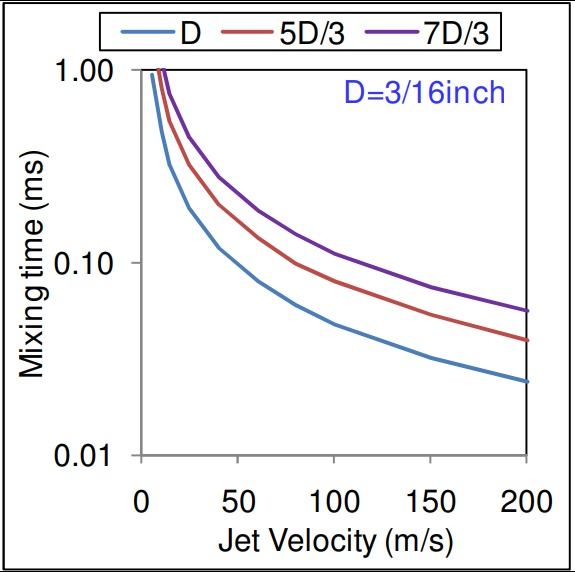
\includegraphics[width=0.97\textwidth]{Chapter3/Images/MixingTime.jpeg}
        \subcaption{Turbulent mixing time with variation of diameter and jet velocity \cite{VAThesis2011}.}
        \label{fig:mixingTime}
    \end{subfigure}
\hfill
    \begin{subfigure}[t]{0.3\textwidth}
        \centering
        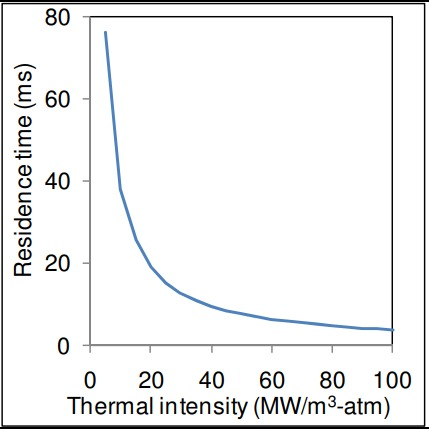
\includegraphics[width=0.97\textwidth]{Chapter3/Images/residenceTimeVsIntensity.jpeg}
        \subcaption{Residence time variation.}
        \label{fig:residenceTimeVsIntensity}
    \end{subfigure}
\hfill
    \begin{subfigure}[t]{0.3\textwidth}
        \centering
        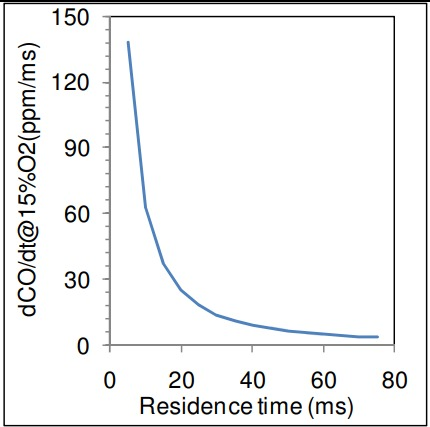
\includegraphics[width=0.97\textwidth]{Chapter3/Images/conversionRateCOtoCo2.jpeg}
        \subcaption{conversion rate CO to CO$_2$.}
        \label{fig:conversionRateCOtoCo2}
    \end{subfigure}
\caption{Turbulent mixing time and residence time plots.}
\label{fig:residenceTimePlots}
\end{figure*}
